\hypertarget{group__distance}{
\section{Distancias}
\label{group__distance}\index{Distancias@{Distancias}}
}


\subsection{Descripci\'{o}n detallada}
Para el projecto utilizamos la definicion de distancia Euclidiana, donde la distancia entre dos objetos es la longitud de la recta mas cercana que los toca. 

\subsection*{Archivos}
\begin{CompactItemize}
\item 
archivo \hyperlink{distance_8h}{distance.h}
\item 
archivo \hyperlink{distance_8c}{distance.c}
\end{CompactItemize}
\subsection*{Funciones}
\begin{CompactItemize}
\item 
float \hyperlink{group__distance_g3b2b03f846e6b587be683ec8b853e774_g3b2b03f846e6b587be683ec8b853e774}{distance\_\-pointpoint} (\hyperlink{struct__point}{point} $\ast$a, \hyperlink{struct__point}{point} $\ast$b)
\item 
float \hyperlink{group__distance_g69a59a49134b784b0c8797e0e83e7c40_g69a59a49134b784b0c8797e0e83e7c40}{distance\_\-pointline} (\hyperlink{struct__point}{point} $\ast$f, \hyperlink{struct__line}{line} $\ast$l, int $\ast$seg)
\item 
float \hyperlink{group__distance_g25716e8d1c8abaf08903bbcd08b8d6e5_g25716e8d1c8abaf08903bbcd08b8d6e5}{distance\_\-pointpolygon} (\hyperlink{struct__point}{point} $\ast$f, \hyperlink{struct__polygon}{polygon} $\ast$p, \hyperlink{struct__line}{line} $\ast$ref)
\item 
float \hyperlink{group__distance_gc837f0084791f42936ade857a0cce3af_gc837f0084791f42936ade857a0cce3af}{distance\_\-pointpolygonholes} (\hyperlink{struct__point}{point} $\ast$f, \hyperlink{struct__polygon__holes}{polygon\_\-holes} $\ast$p, \hyperlink{struct__line}{line} $\ast$ref)
\end{CompactItemize}


\subsection{Documentaci\'{o}n de las funciones}
\hypertarget{group__distance_g69a59a49134b784b0c8797e0e83e7c40_g69a59a49134b784b0c8797e0e83e7c40}{
\index{distance@{distance}!distance_pointline@{distance\_\-pointline}}
\index{distance_pointline@{distance\_\-pointline}!distance@{distance}}
\subsubsection[distance\_\-pointline]{\setlength{\rightskip}{0pt plus 5cm}float distance\_\-pointline (\hyperlink{struct__point}{point} $\ast$ {\em f}, \hyperlink{struct__line}{line} $\ast$ {\em l}, int $\ast$ {\em seg})}}
\label{group__distance_g69a59a49134b784b0c8797e0e83e7c40_g69a59a49134b784b0c8797e0e83e7c40}


La funcion calcula la distancia entre un punto un segmento de linea, se pueden dar dos casos:\begin{itemize}
\item La perpendicular del punto a la recta intersecta el segmento de recta, en esta caso la distancia es la longitud del punto al punto de interseccion de la recta con la perpendicular que pasa por el punto\end{itemize}


\begin{itemize}
\item La perpendicular del punto a la recta no intersecta el segmente, en este caso la distancia entre el punto y la recta es igual a la minima distancia entre el punto y los puntos extremos del segmento de recta.\end{itemize}


\begin{Desc}
\item[Par\'{a}metros:]
\begin{description}
\item[\mbox{$\leftarrow$} {\em f}]Punto en 2 dimensiones \item[\mbox{$\leftarrow$} {\em l}]Segmento de recta que tiene definido los dos puntos extremos \item[\mbox{$\rightarrow$} {\em seg}]Indica cual fue la refencia para tomar la distancia puede tomar tres valores:0 cuando la distancia es respecto a la perpendicular de la linea, 1 cuando la distancia es respecto al punto extremo 1 y 2 cuando la distancia es respecto al punto extremo 2 \end{description}
\end{Desc}
\begin{Desc}
\item[Devuelve:]La distancia entre el segmento de recta y el punto \end{Desc}


Definici\'{o}n en la l\'{\i}nea 54 del archivo distance.c.

\begin{Code}\begin{verbatim}55 {
56     if(point_dot(&(l->v1),&(l->v2),f) > 0)
57     {
58         *seg = 2;
59         return distance_pointpoint(&(l->v2),f);
60     }
61 
62     if(point_dot(&(l->v2),&(l->v1),f) > 0)
63     {
64         *seg =1;
65         return distance_pointpoint(&(l->v1),f);
66     }
67 
68     *seg =0;
69     return fabsf(point_cross(&(l->v1),&(l->v2),f) / distance_pointpoint(&(l->v1),&(l->v2)));
70 }
\end{verbatim}\end{Code}




Gr\'{a}fico de llamadas para esta funci\'{o}n:\begin{figure}[H]
\begin{center}
\leavevmode
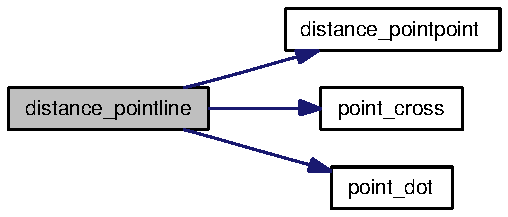
\includegraphics[width=140pt]{group__distance_g69a59a49134b784b0c8797e0e83e7c40_g69a59a49134b784b0c8797e0e83e7c40_cgraph}
\end{center}
\end{figure}


Here is the caller graph for this function:\begin{figure}[H]
\begin{center}
\leavevmode
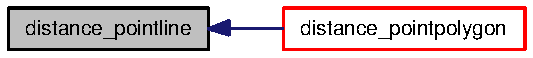
\includegraphics[width=146pt]{group__distance_g69a59a49134b784b0c8797e0e83e7c40_g69a59a49134b784b0c8797e0e83e7c40_icgraph}
\end{center}
\end{figure}
\hypertarget{group__distance_g3b2b03f846e6b587be683ec8b853e774_g3b2b03f846e6b587be683ec8b853e774}{
\index{distance@{distance}!distance_pointpoint@{distance\_\-pointpoint}}
\index{distance_pointpoint@{distance\_\-pointpoint}!distance@{distance}}
\subsubsection[distance\_\-pointpoint]{\setlength{\rightskip}{0pt plus 5cm}float distance\_\-pointpoint (\hyperlink{struct__point}{point} $\ast$ {\em a}, \hyperlink{struct__point}{point} $\ast$ {\em b})}}
\label{group__distance_g3b2b03f846e6b587be683ec8b853e774_g3b2b03f846e6b587be683ec8b853e774}


La funcion compara la distancia entre dos puntos la formula para esto es: $\sqrt{(x_2 - x_1)^2 + (y_2 - y_1)^2}$

\begin{Desc}
\item[Par\'{a}metros:]
\begin{description}
\item[\mbox{$\leftarrow$} {\em a}]Punto en 2 dimensiones \item[\mbox{$\leftarrow$} {\em b}]Punto en 2 dimensiones \end{description}
\end{Desc}
\begin{Desc}
\item[Devuelve:]La distancia entre los puntos \end{Desc}


Definici\'{o}n en la l\'{\i}nea 29 del archivo distance.c.

\begin{Code}\begin{verbatim}30 {
31     return sqrt(powf(a->x - b->x,2.0)+powf(a->y - b->y,2.0));
32 }
\end{verbatim}\end{Code}




Here is the caller graph for this function:\begin{figure}[H]
\begin{center}
\leavevmode
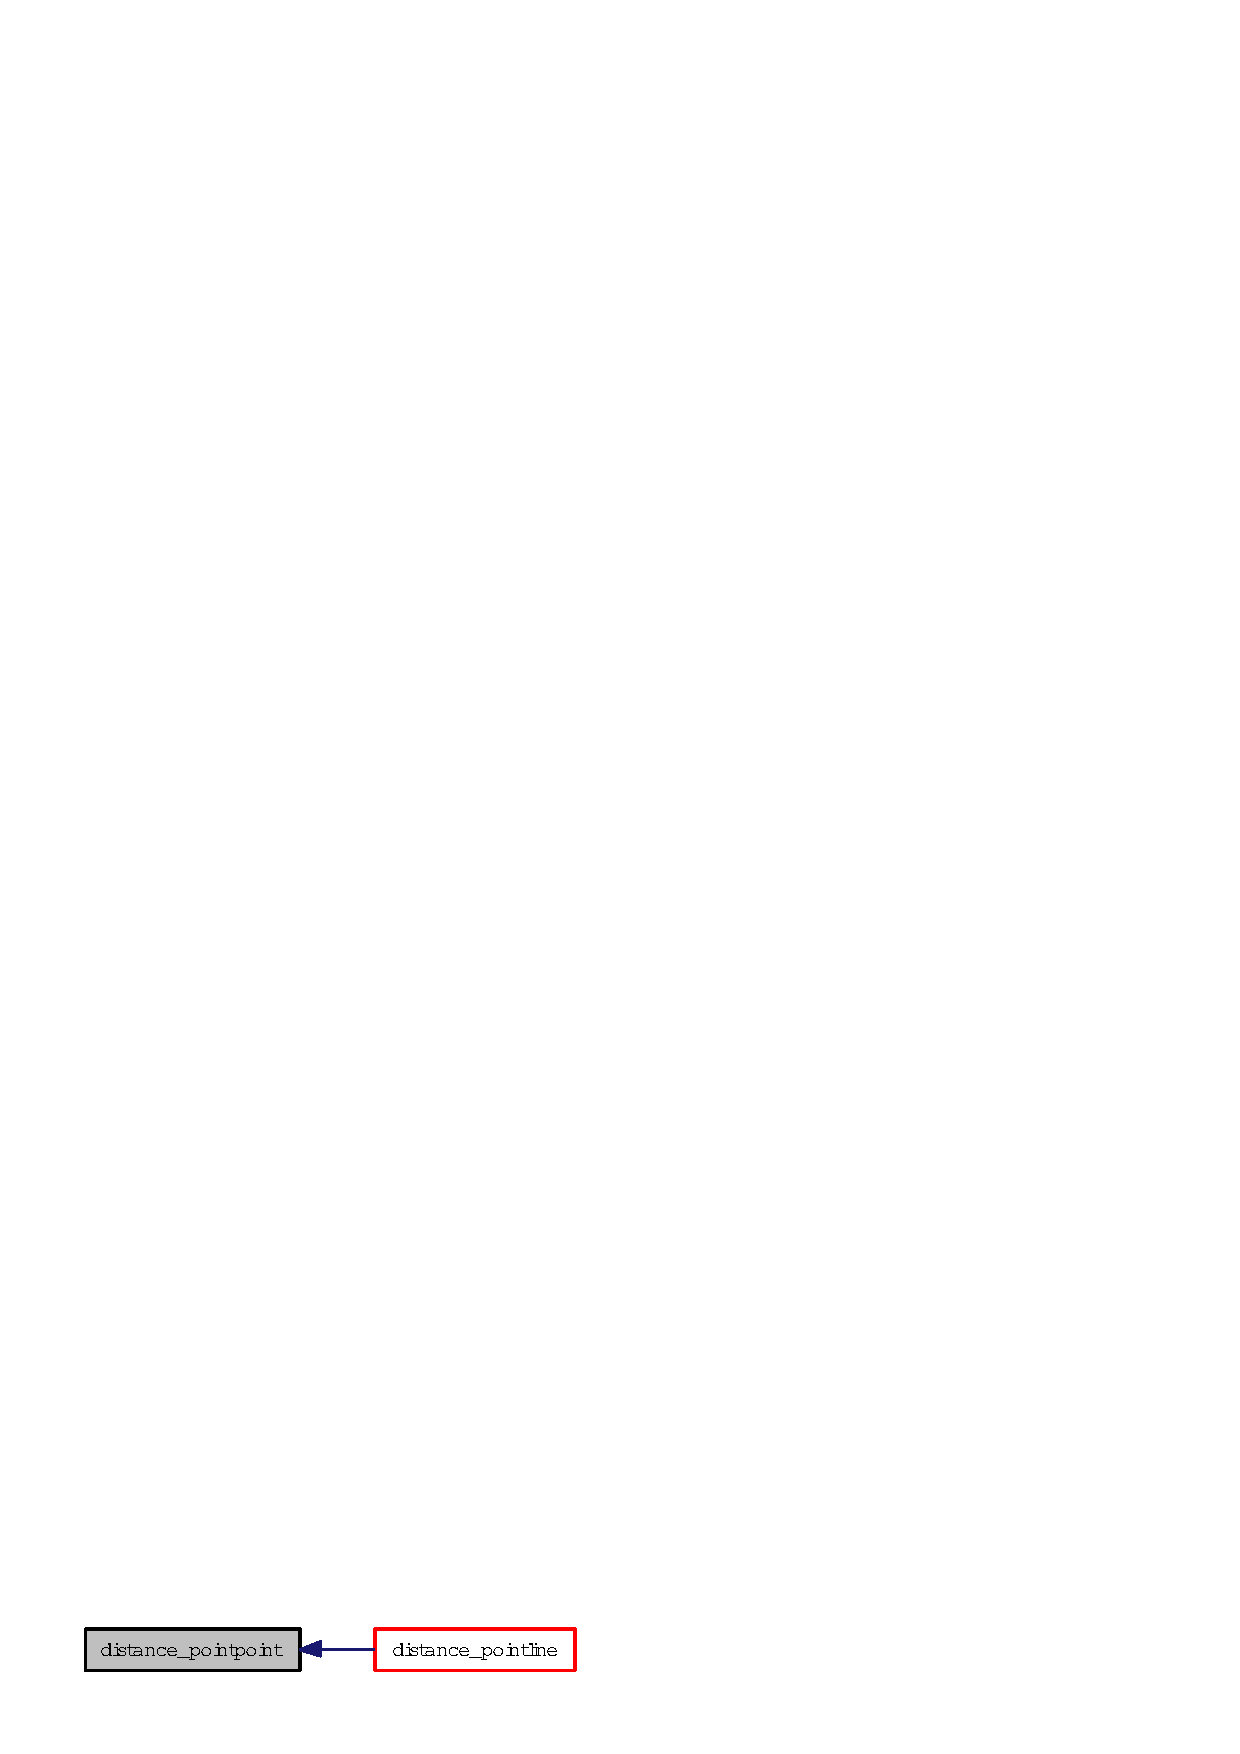
\includegraphics[width=140pt]{group__distance_g3b2b03f846e6b587be683ec8b853e774_g3b2b03f846e6b587be683ec8b853e774_icgraph}
\end{center}
\end{figure}
\hypertarget{group__distance_g25716e8d1c8abaf08903bbcd08b8d6e5_g25716e8d1c8abaf08903bbcd08b8d6e5}{
\index{distance@{distance}!distance_pointpolygon@{distance\_\-pointpolygon}}
\index{distance_pointpolygon@{distance\_\-pointpolygon}!distance@{distance}}
\subsubsection[distance\_\-pointpolygon]{\setlength{\rightskip}{0pt plus 5cm}float distance\_\-pointpolygon (\hyperlink{struct__point}{point} $\ast$ {\em f}, \hyperlink{struct__polygon}{polygon} $\ast$ {\em p}, \hyperlink{struct__line}{line} $\ast$ {\em ref})}}
\label{group__distance_g25716e8d1c8abaf08903bbcd08b8d6e5_g25716e8d1c8abaf08903bbcd08b8d6e5}


La funcion calcula la distancia entre un punto y el borde de un poligono simple, para esto calcula la distancia del punto contra todos los segmentos de linea que conforma el poligono y retorna la menor distancia, esta funcion no tiene consideracion si el punto esta adentro o afuera del poligono porque calcula la distancia al borde.

\begin{Desc}
\item[Par\'{a}metros:]
\begin{description}
\item[\mbox{$\leftarrow$} {\em f}]Punto en 2 dimensiones \item[\mbox{$\leftarrow$} {\em p}]Poligono simple \item[\mbox{$\rightarrow$} {\em ref}]Escribe en la memoria el segmento de recta que define la menor distancia entre el poligono y el punto, si la distancia fue tomada respecto a un punto extremo, entonces el segmento de recta es un punto, el extremo. \end{description}
\end{Desc}
\begin{Desc}
\item[Devuelve:]La distancia entre el punto y el poligono \end{Desc}


Definici\'{o}n en la l\'{\i}nea 87 del archivo distance.c.

\begin{Code}\begin{verbatim}88 {
89     int seg,i;
90     float min=FLT_MAX;
91 
92     for (i=0;i<p->nvertices;i++)
93     {
94         float d;
95         line l;
96 
97         l.v1=p->v[i];
98         l.v2=p->v[(i+1)%(p->nvertices)];
99         d=distance_pointline(f,&l,&seg);
100         if (i==0 || min>d)
101         {
102             min = d;
103             if (ref!=NULL)
104             {
105                 switch (seg)
106                 {
107                     case 0:
108                     ref->v1 = l.v1;
109                     ref->v2 = l.v2;
110                     break;
111                     case 1:
112                     ref->v1 = l.v1;
113                     ref->v2 = l.v1;
114                     break;
115                     case 2:
116                     ref->v1 = l.v2;
117                     ref->v2 = l.v2;
118                     break;
119                 }
120             }
121         }
122     }
123     return min;
124 }
\end{verbatim}\end{Code}




Gr\'{a}fico de llamadas para esta funci\'{o}n:\begin{figure}[H]
\begin{center}
\leavevmode
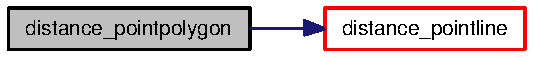
\includegraphics[width=146pt]{group__distance_g25716e8d1c8abaf08903bbcd08b8d6e5_g25716e8d1c8abaf08903bbcd08b8d6e5_cgraph}
\end{center}
\end{figure}


Here is the caller graph for this function:\begin{figure}[H]
\begin{center}
\leavevmode
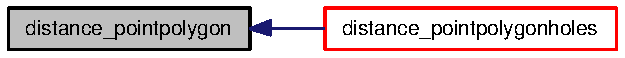
\includegraphics[width=168pt]{group__distance_g25716e8d1c8abaf08903bbcd08b8d6e5_g25716e8d1c8abaf08903bbcd08b8d6e5_icgraph}
\end{center}
\end{figure}
\hypertarget{group__distance_gc837f0084791f42936ade857a0cce3af_gc837f0084791f42936ade857a0cce3af}{
\index{distance@{distance}!distance_pointpolygonholes@{distance\_\-pointpolygonholes}}
\index{distance_pointpolygonholes@{distance\_\-pointpolygonholes}!distance@{distance}}
\subsubsection[distance\_\-pointpolygonholes]{\setlength{\rightskip}{0pt plus 5cm}float distance\_\-pointpolygonholes (\hyperlink{struct__point}{point} $\ast$ {\em f}, \hyperlink{struct__polygon__holes}{polygon\_\-holes} $\ast$ {\em p}, \hyperlink{struct__line}{line} $\ast$ {\em ref})}}
\label{group__distance_gc837f0084791f42936ade857a0cce3af_gc837f0084791f42936ade857a0cce3af}


La funcion calcula la distancia entre un punto y un poligono con huecos, para esto calcula la distancia del punto con el borde del poligono y posteriormente con cada uno de los huecos de este, seleccionado la distancia minima \begin{Desc}
\item[Par\'{a}metros:]
\begin{description}
\item[\mbox{$\leftarrow$} {\em f}]Punto en 2 dimensiones \item[\mbox{$\leftarrow$} {\em p}]Poligono con huecos \item[\mbox{$\rightarrow$} {\em ref}]Escribe en la memoria el segmento de recta que define la menor distancia entre el poligono y sus huecos con el punto, si la distancia fue tomada respecto a un punto extremo, entonces el segmento de recta es un punto, el extremo. \end{description}
\end{Desc}
\begin{Desc}
\item[Devuelve:]La distancia entre un punto y un poligono con huecos \end{Desc}


Definici\'{o}n en la l\'{\i}nea 139 del archivo distance.c.

\begin{Code}\begin{verbatim}140 {
141     int i;
142     float min;
143 
144     min = distance_pointpolygon(f,p->p,ref);
145     for (i=0;i<p->nholes;i++)
146     {
147         float min2;
148         line ref2;
149         min2 = distance_pointpolygon(f,&(p->h[i]),&ref2);
150         if (min2 < min)
151         {
152             min = min2;
153             if (ref!=NULL)
154             {
155                 ref->v1 = ref2.v1;
156                 ref->v2 = ref2.v2;
157             }
158         }
159     }
160     return min;
161 }
\end{verbatim}\end{Code}




Gr\'{a}fico de llamadas para esta funci\'{o}n:\begin{figure}[H]
\begin{center}
\leavevmode
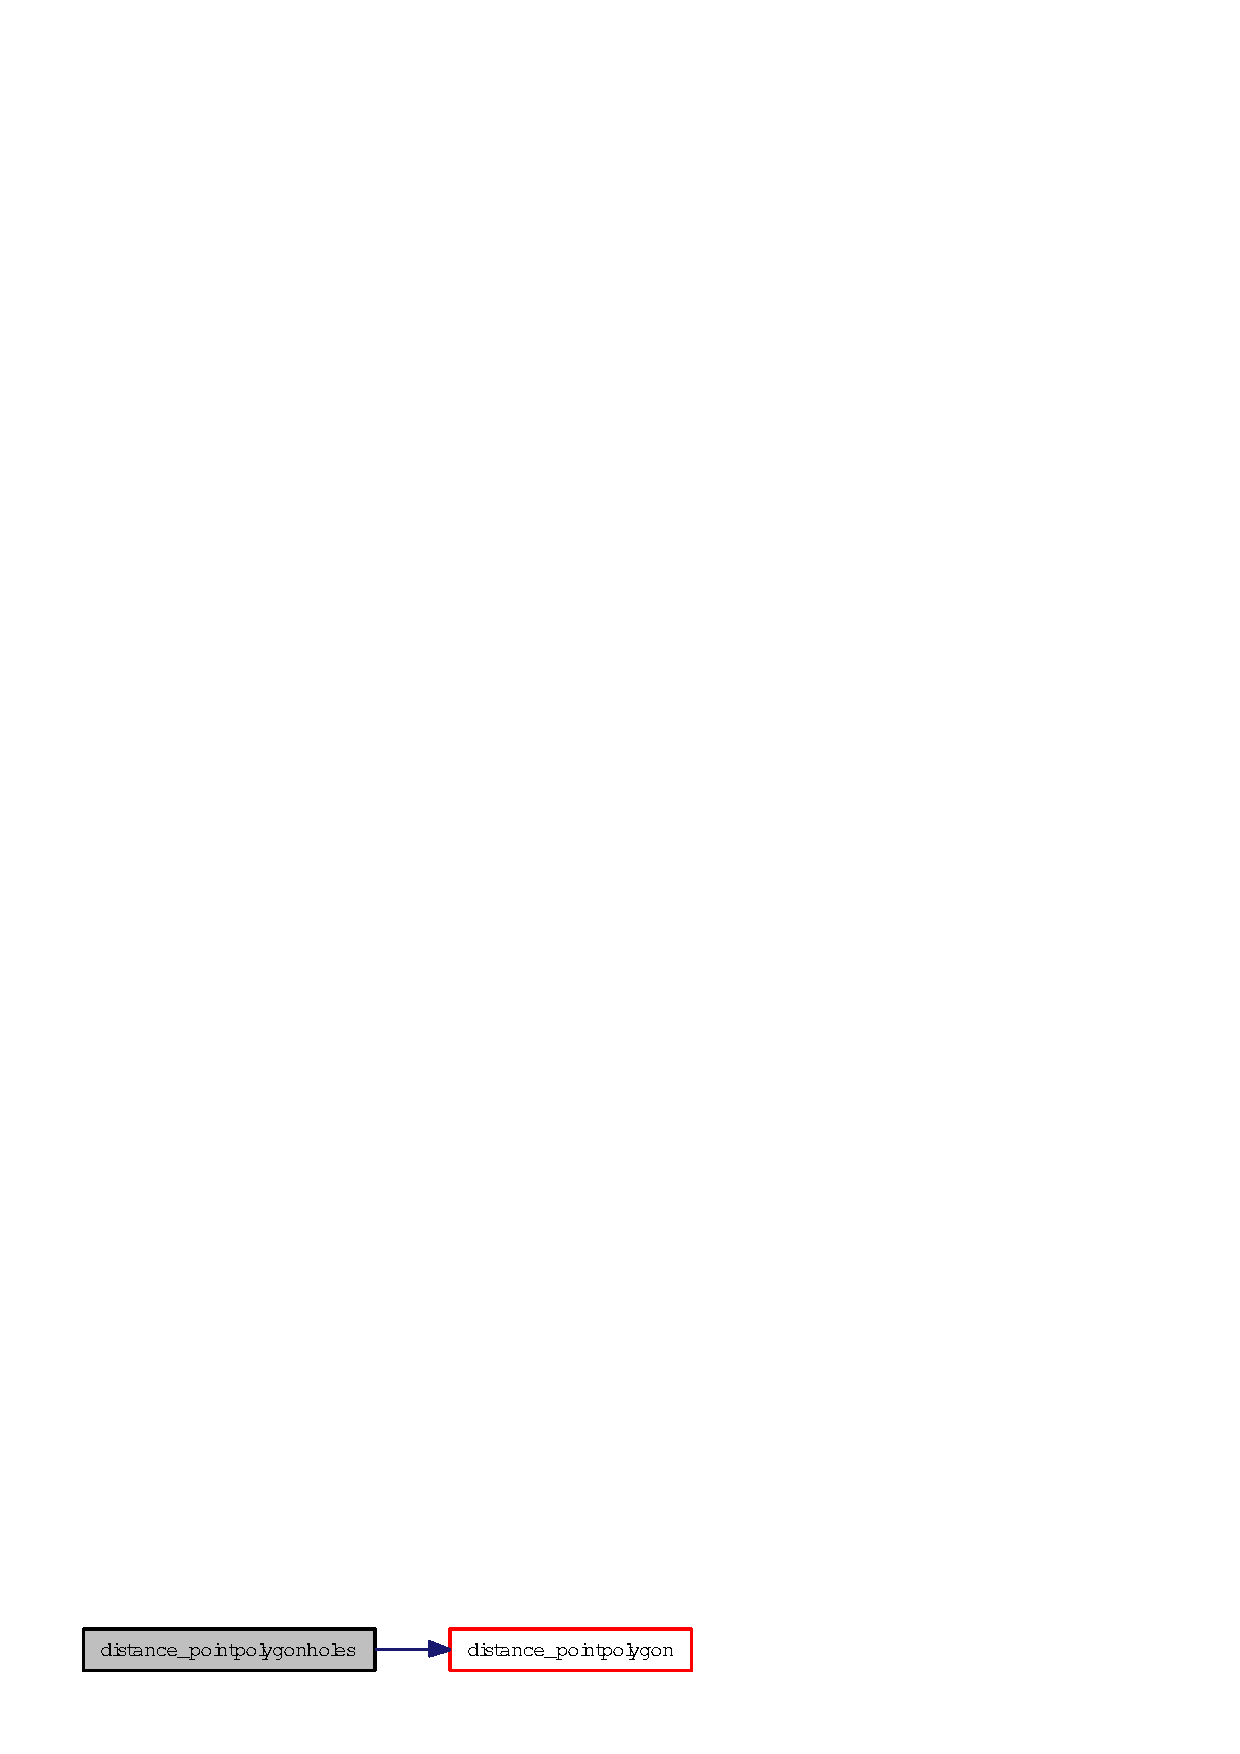
\includegraphics[width=168pt]{group__distance_gc837f0084791f42936ade857a0cce3af_gc837f0084791f42936ade857a0cce3af_cgraph}
\end{center}
\end{figure}


Here is the caller graph for this function:\begin{figure}[H]
\begin{center}
\leavevmode
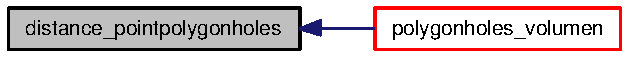
\includegraphics[width=169pt]{group__distance_gc837f0084791f42936ade857a0cce3af_gc837f0084791f42936ade857a0cce3af_icgraph}
\end{center}
\end{figure}
